\documentclass[1p]{elsarticle_modified}
%\bibliographystyle{elsarticle-num}

%\usepackage[colorlinks]{hyperref}
%\usepackage{abbrmath_seonhwa} %\Abb, \Ascr, \Acal ,\Abf, \Afrak
\usepackage{amsfonts}
\usepackage{amssymb}
\usepackage{amsmath}
\usepackage{amsthm}
\usepackage{scalefnt}
\usepackage{amsbsy}
\usepackage{kotex}
\usepackage{caption}
\usepackage{subfig}
\usepackage{color}
\usepackage{graphicx}
\usepackage{xcolor} %% white, black, red, green, blue, cyan, magenta, yellow
\usepackage{float}
\usepackage{setspace}
\usepackage{hyperref}

\usepackage{tikz}
\usetikzlibrary{arrows}

\usepackage{multirow}
\usepackage{array} % fixed length table
\usepackage{hhline}

%%%%%%%%%%%%%%%%%%%%%
\makeatletter
\renewcommand*\env@matrix[1][\arraystretch]{%
	\edef\arraystretch{#1}%
	\hskip -\arraycolsep
	\let\@ifnextchar\new@ifnextchar
	\array{*\c@MaxMatrixCols c}}
\makeatother %https://tex.stackexchange.com/questions/14071/how-can-i-increase-the-line-spacing-in-a-matrix
%%%%%%%%%%%%%%%

\usepackage[normalem]{ulem}

\newcommand{\msout}[1]{\ifmmode\text{\sout{\ensuremath{#1}}}\else\sout{#1}\fi}
%SOURCE: \msout is \stkout macro in https://tex.stackexchange.com/questions/20609/strikeout-in-math-mode

\newcommand{\cancel}[1]{
	\ifmmode
	{\color{red}\msout{#1}}
	\else
	{\color{red}\sout{#1}}
	\fi
}

\newcommand{\add}[1]{
	{\color{blue}\uwave{#1}}
}

\newcommand{\replace}[2]{
	\ifmmode
	{\color{red}\msout{#1}}{\color{blue}\uwave{#2}}
	\else
	{\color{red}\sout{#1}}{\color{blue}\uwave{#2}}
	\fi
}

\newcommand{\Sol}{\mathcal{S}} %segment
\newcommand{\D}{D} %diagram
\newcommand{\A}{\mathcal{A}} %arc


%%%%%%%%%%%%%%%%%%%%%%%%%%%%%5 test

\def\sl{\operatorname{\textup{SL}}(2,\Cbb)}
\def\psl{\operatorname{\textup{PSL}}(2,\Cbb)}
\def\quan{\mkern 1mu \triangleright \mkern 1mu}

\theoremstyle{definition}
\newtheorem{thm}{Theorem}[section]
\newtheorem{prop}[thm]{Proposition}
\newtheorem{lem}[thm]{Lemma}
\newtheorem{ques}[thm]{Question}
\newtheorem{cor}[thm]{Corollary}
\newtheorem{defn}[thm]{Definition}
\newtheorem{exam}[thm]{Example}
\newtheorem{rmk}[thm]{Remark}
\newtheorem{alg}[thm]{Algorithm}

\newcommand{\I}{\sqrt{-1}}
\begin{document}

%\begin{frontmatter}
%
%\title{Boundary parabolic representations of knots up to 8 crossings}
%
%%% Group authors per affiliation:
%\author{Yunhi Cho} 
%\address{Department of Mathematics, University of Seoul, Seoul, Korea}
%\ead{yhcho@uos.ac.kr}
%
%
%\author{Seonhwa Kim} %\fnref{s_kim}}
%\address{Center for Geometry and Physics, Institute for Basic Science, Pohang, 37673, Korea}
%\ead{ryeona17@ibs.re.kr}
%
%\author{Hyuk Kim}
%\address{Department of Mathematical Sciences, Seoul National University, Seoul 08826, Korea}
%\ead{hyukkim@snu.ac.kr}
%
%\author{Seokbeom Yoon}
%\address{Department of Mathematical Sciences, Seoul National University, Seoul, 08826,  Korea}
%\ead{sbyoon15@snu.ac.kr}
%
%\begin{abstract}
%We find all boundary parabolic representation of knots up to 8 crossings.
%
%\end{abstract}
%\begin{keyword}
%    \MSC[2010] 57M25 
%\end{keyword}
%
%\end{frontmatter}

%\linenumbers
%\tableofcontents
%
\newcommand\colored[1]{\textcolor{white}{\rule[-0.35ex]{0.8em}{1.4ex}}\kern-0.8em\color{red} #1}%
%\newcommand\colored[1]{\textcolor{white}{ #1}\kern-2.17ex	\textcolor{white}{ #1}\kern-1.81ex	\textcolor{white}{ #1}\kern-2.15ex\color{red}#1	}

{\Large $\underline{12a_{1260}~(K12a_{1260})}$}

\setlength{\tabcolsep}{10pt}
\renewcommand{\arraystretch}{1.6}
\vspace{1cm}\begin{tabular}{m{100pt}>{\centering\arraybackslash}m{274pt}}
\multirow{5}{120pt}{
	\centering
	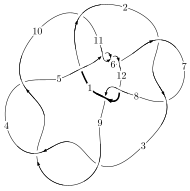
\includegraphics[width=112pt]{../../../GIT/diagram.site/Diagrams/png/2061_12a_1260.png}\\
\ \ \ A knot diagram\footnotemark}&
\allowdisplaybreaks
\textbf{Linearized knot diagam} \\
\cline{2-2}
 &
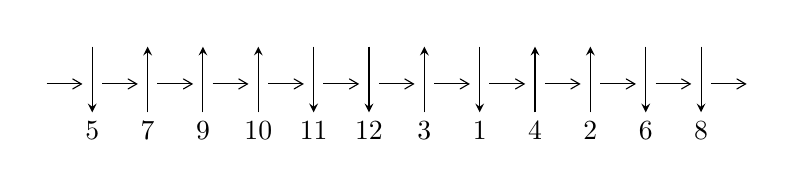
\begin{tikzpicture}[x=20pt, y=17pt]
	% nodes
	\node (C0) at (0, 0) {};
	\node (C1) at (1, 0) {};
	\node (C1U) at (1, +1) {};
	\node (C1D) at (1, -1) {5};

	\node (C2) at (2, 0) {};
	\node (C2U) at (2, +1) {};
	\node (C2D) at (2, -1) {7};

	\node (C3) at (3, 0) {};
	\node (C3U) at (3, +1) {};
	\node (C3D) at (3, -1) {9};

	\node (C4) at (4, 0) {};
	\node (C4U) at (4, +1) {};
	\node (C4D) at (4, -1) {10};

	\node (C5) at (5, 0) {};
	\node (C5U) at (5, +1) {};
	\node (C5D) at (5, -1) {11};

	\node (C6) at (6, 0) {};
	\node (C6U) at (6, +1) {};
	\node (C6D) at (6, -1) {12};

	\node (C7) at (7, 0) {};
	\node (C7U) at (7, +1) {};
	\node (C7D) at (7, -1) {3};

	\node (C8) at (8, 0) {};
	\node (C8U) at (8, +1) {};
	\node (C8D) at (8, -1) {1};

	\node (C9) at (9, 0) {};
	\node (C9U) at (9, +1) {};
	\node (C9D) at (9, -1) {4};

	\node (C10) at (10, 0) {};
	\node (C10U) at (10, +1) {};
	\node (C10D) at (10, -1) {2};

	\node (C11) at (11, 0) {};
	\node (C11U) at (11, +1) {};
	\node (C11D) at (11, -1) {6};

	\node (C12) at (12, 0) {};
	\node (C12U) at (12, +1) {};
	\node (C12D) at (12, -1) {8};
	\node (C13) at (13, 0) {};

	% arrows
	\draw[->,>={angle 60}]
	(C0) edge (C1) (C1) edge (C2) (C2) edge (C3) (C3) edge (C4) (C4) edge (C5) (C5) edge (C6) (C6) edge (C7) (C7) edge (C8) (C8) edge (C9) (C9) edge (C10) (C10) edge (C11) (C11) edge (C12) (C12) edge (C13) ;	\draw[->,>=stealth]
	(C1U) edge (C1D) (C2D) edge (C2U) (C3D) edge (C3U) (C4D) edge (C4U) (C5U) edge (C5D) (C6U) edge (C6D) (C7D) edge (C7U) (C8U) edge (C8D) (C9D) edge (C9U) (C10D) edge (C10U) (C11U) edge (C11D) (C12U) edge (C12D) ;
	\end{tikzpicture} \\
\hhline{~~} \\& 
\textbf{Solving Sequence} \\ \cline{2-2} 
 &
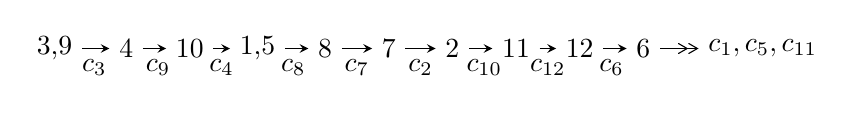
\begin{tikzpicture}[x=23pt, y=7pt]
	% node
	\node (A0) at (-1/8, 0) {3,9};
	\node (A1) at (1, 0) {4};
	\node (A2) at (2, 0) {10};
	\node (A3) at (49/16, 0) {1,5};
	\node (A4) at (33/8, 0) {8};
	\node (A5) at (41/8, 0) {7};
	\node (A6) at (49/8, 0) {2};
	\node (A7) at (57/8, 0) {11};
	\node (A8) at (65/8, 0) {12};
	\node (A9) at (73/8, 0) {6};
	\node (C1) at (1/2, -1) {$c_{3}$};
	\node (C2) at (3/2, -1) {$c_{9}$};
	\node (C3) at (5/2, -1) {$c_{4}$};
	\node (C4) at (29/8, -1) {$c_{8}$};
	\node (C5) at (37/8, -1) {$c_{7}$};
	\node (C6) at (45/8, -1) {$c_{2}$};
	\node (C7) at (53/8, -1) {$c_{10}$};
	\node (C8) at (61/8, -1) {$c_{12}$};
	\node (C9) at (69/8, -1) {$c_{6}$};
	\node (A10) at (11, 0) {$c_{1},c_{5},c_{11}$};

	% edge
	\draw[->,>=stealth]	
	(A0) edge (A1) (A1) edge (A2) (A2) edge (A3) (A3) edge (A4) (A4) edge (A5) (A5) edge (A6) (A6) edge (A7) (A7) edge (A8) (A8) edge (A9) ;
	\draw[->>,>={angle 60}]	
	(A9) edge (A10);
\end{tikzpicture} \\ 

\end{tabular} \\

\footnotetext{
The image of knot diagram is generated by the software ``\textbf{Draw programme}" developed by Andrew Bartholomew(\url{http://www.layer8.co.uk/maths/draw/index.htm\#Running-draw}), where we modified some parts for our purpose(\url{https://github.com/CATsTAILs/LinksPainter}).
}\phantom \\ \newline 
\centering \textbf{Ideals for irreducible components\footnotemark of $X_{\text{par}}$} 
 
\begin{align*}
I^u_{1}&=\langle 
-4.25260\times10^{169} u^{87}+4.64928\times10^{169} u^{86}+\cdots+1.00310\times10^{170} b-5.41733\times10^{169},\\
\phantom{I^u_{1}}&\phantom{= \langle  }-1.51686\times10^{169} u^{87}-8.93383\times10^{169} u^{86}+\cdots+1.00310\times10^{170} a-4.70692\times10^{171},\\
\phantom{I^u_{1}}&\phantom{= \langle  }u^{88}-45 u^{86}+\cdots+44 u-1\rangle \\
I^u_{2}&=\langle 
-29 u^{15}-34 u^{14}+\cdots+73 b-87,\;-82 u^{15}+70 u^{14}+\cdots+73 a+119,\\
\phantom{I^u_{2}}&\phantom{= \langle  }u^{16}-9 u^{14}+34 u^{12}- u^{11}-72 u^{10}+7 u^9+95 u^8-19 u^7-76 u^6+24 u^5+26 u^4-12 u^3+4 u^2-1\rangle \\
I^u_{3}&=\langle 
b,\;a-1,\;u+1\rangle \\
I^u_{4}&=\langle 
b-1,\;a,\;u+1\rangle \\
I^u_{5}&=\langle 
b+1,\;a-1,\;u-1\rangle \\
\\
I^v_{1}&=\langle 
a,\;b-1,\;v+1\rangle \\
\end{align*}
\raggedright * 6 irreducible components of $\dim_{\mathbb{C}}=0$, with total 108 representations.\\
\footnotetext{All coefficients of polynomials are rational numbers. But the coefficients are sometimes approximated in decimal forms when there is not enough margin.}
\newpage
\renewcommand{\arraystretch}{1}
\centering \section*{I. $I^u_{1}= \langle -4.25\times10^{169} u^{87}+4.65\times10^{169} u^{86}+\cdots+1.00\times10^{170} b-5.42\times10^{169},\;-1.52\times10^{169} u^{87}-8.93\times10^{169} u^{86}+\cdots+1.00\times10^{170} a-4.71\times10^{171},\;u^{88}-45 u^{86}+\cdots+44 u-1 \rangle$}
\flushleft \textbf{(i) Arc colorings}\\
\begin{tabular}{m{7pt} m{180pt} m{7pt} m{180pt} }
\flushright $a_{3}=$&$\begin{pmatrix}1\\0\end{pmatrix}$ \\
\flushright $a_{9}=$&$\begin{pmatrix}0\\u\end{pmatrix}$ \\
\flushright $a_{4}=$&$\begin{pmatrix}1\\- u^2\end{pmatrix}$ \\
\flushright $a_{10}=$&$\begin{pmatrix}u\\- u^3+u\end{pmatrix}$ \\
\flushright $a_{1}=$&$\begin{pmatrix}0.151218 u^{87}+0.890626 u^{86}+\cdots+92.0941 u+46.9239\\0.423948 u^{87}-0.463494 u^{86}+\cdots+16.2841 u+0.540062\end{pmatrix}$ \\
\flushright $a_{5}=$&$\begin{pmatrix}- u^2+1\\u^4-2 u^2\end{pmatrix}$ \\
\flushright $a_{8}=$&$\begin{pmatrix}0.289659 u^{87}+1.45974 u^{86}+\cdots+185.969 u+46.5951\\0.352924 u^{87}-0.532037 u^{86}+\cdots+16.0338 u+0.601752\end{pmatrix}$ \\
\flushright $a_{7}=$&$\begin{pmatrix}-0.0632654 u^{87}+1.99177 u^{86}+\cdots+169.935 u+45.9934\\0.352924 u^{87}-0.532037 u^{86}+\cdots+16.0338 u+0.601752\end{pmatrix}$ \\
\flushright $a_{2}=$&$\begin{pmatrix}-0.232052 u^{87}+1.30060 u^{86}+\cdots+80.2068 u+46.2469\\0.257568 u^{87}-0.257637 u^{86}+\cdots+11.0024 u+0.658405\end{pmatrix}$ \\
\flushright $a_{11}=$&$\begin{pmatrix}2.82460 u^{87}-2.45778 u^{86}+\cdots+259.385 u+42.0583\\-0.158379 u^{87}+0.283717 u^{86}+\cdots-2.29390 u+0.979181\end{pmatrix}$ \\
\flushright $a_{12}=$&$\begin{pmatrix}2.32651 u^{87}-2.66880 u^{86}+\cdots+154.491 u-6.36215\\-0.123834 u^{87}+0.152593 u^{86}+\cdots+0.0420976 u-0.0772851\end{pmatrix}$ \\
\flushright $a_{6}=$&$\begin{pmatrix}2.90389 u^{87}-3.07386 u^{86}+\cdots+116.798 u+43.8565\\-0.0923931 u^{87}+0.118452 u^{86}+\cdots-3.90791 u+0.961875\end{pmatrix}$\\&\end{tabular}
\flushleft \textbf{(ii) Obstruction class $= -1$}\\~\\
\flushleft \textbf{(iii) Cusp Shapes $= 1.12053 u^{87}-1.26633 u^{86}+\cdots+131.631 u-8.78215$}\\~\\
\newpage\renewcommand{\arraystretch}{1}
\flushleft \textbf{(iv) u-Polynomials at the component}\newline \\
\begin{tabular}{m{50pt}|m{274pt}}
Crossings & \hspace{64pt}u-Polynomials at each crossing \\
\hline $$\begin{aligned}c_{1}\end{aligned}$$&$\begin{aligned}
&u^{88}+8 u^{87}+\cdots+24 u-7
\end{aligned}$\\
\hline $$\begin{aligned}c_{2},c_{7}\end{aligned}$$&$\begin{aligned}
&u^{88}+2 u^{87}+\cdots+2042 u+301
\end{aligned}$\\
\hline $$\begin{aligned}c_{3},c_{4},c_{9}\end{aligned}$$&$\begin{aligned}
&u^{88}-45 u^{86}+\cdots-44 u-1
\end{aligned}$\\
\hline $$\begin{aligned}c_{5},c_{6},c_{11}\end{aligned}$$&$\begin{aligned}
&u^{88}-45 u^{86}+\cdots+44 u-1
\end{aligned}$\\
\hline $$\begin{aligned}c_{8},c_{12}\end{aligned}$$&$\begin{aligned}
&u^{88}-2 u^{87}+\cdots-2042 u+301
\end{aligned}$\\
\hline $$\begin{aligned}c_{10}\end{aligned}$$&$\begin{aligned}
&u^{88}-8 u^{87}+\cdots-24 u-7
\end{aligned}$\\
\hline
\end{tabular}\\~\\
\newpage\renewcommand{\arraystretch}{1}
\flushleft \textbf{(v) Riley Polynomials at the component}\newline \\
\begin{tabular}{m{50pt}|m{274pt}}
Crossings & \hspace{64pt}Riley Polynomials at each crossing \\
\hline $$\begin{aligned}c_{1},c_{10}\end{aligned}$$&$\begin{aligned}
&y^{88}-8 y^{87}+\cdots-8654 y+49
\end{aligned}$\\
\hline $$\begin{aligned}c_{2},c_{7},c_{8}\\c_{12}\end{aligned}$$&$\begin{aligned}
&y^{88}-52 y^{87}+\cdots-2985028 y+90601
\end{aligned}$\\
\hline $$\begin{aligned}c_{3},c_{4},c_{5}\\c_{6},c_{9},c_{11}\end{aligned}$$&$\begin{aligned}
&y^{88}-90 y^{87}+\cdots-2260 y+1
\end{aligned}$\\
\hline
\end{tabular}\\~\\
\newpage\flushleft \textbf{(vi) Complex Volumes and Cusp Shapes}
$$\begin{array}{c|c|c}  
\text{Solutions to }I^u_{1}& \I (\text{vol} + \sqrt{-1}CS) & \text{Cusp shape}\\
 \hline 
\begin{aligned}
u &= \phantom{-}0.544396 + 0.875051 I \\
a &= \phantom{-}0.172978 - 1.352960 I \\
b &= -0.73139 - 1.57973 I\end{aligned}
 & -6.7713 + 12.4764 I & \phantom{-0.000000 } 0 \\ \hline\begin{aligned}
u &= \phantom{-}0.544396 - 0.875051 I \\
a &= \phantom{-}0.172978 + 1.352960 I \\
b &= -0.73139 + 1.57973 I\end{aligned}
 & -6.7713 - 12.4764 I & \phantom{-0.000000 } 0 \\ \hline\begin{aligned}
u &= -0.956317\phantom{ +0.000000I} \\
a &= \phantom{-}0.992268\phantom{ +0.000000I} \\
b &= \phantom{-}0.0789854\phantom{ +0.000000I}\end{aligned}
 & \phantom{-}1.64464\phantom{ +0.000000I} & \phantom{-0.000000 } 0 \\ \hline\begin{aligned}
u &= -0.550886 + 0.922977 I \\
a &= \phantom{-}0.155827 + 1.167370 I \\
b &= -0.80126 + 1.56648 I\end{aligned}
 & \phantom{-0.000000 } -7.97391 I & \phantom{-0.000000 } 0 \\ \hline\begin{aligned}
u &= -0.550886 - 0.922977 I \\
a &= \phantom{-}0.155827 - 1.167370 I \\
b &= -0.80126 - 1.56648 I\end{aligned}
 & \phantom{-0.000000 -}7.97391 I & \phantom{-0.000000 } 0 \\ \hline\begin{aligned}
u &= \phantom{-}1.044190 + 0.280270 I \\
a &= \phantom{-}1.230330 - 0.059806 I \\
b &= \phantom{-}0.217785 - 0.468266 I\end{aligned}
 & -3.22549 - 0.27919 I & \phantom{-0.000000 } 0 \\ \hline\begin{aligned}
u &= \phantom{-}1.044190 - 0.280270 I \\
a &= \phantom{-}1.230330 + 0.059806 I \\
b &= \phantom{-}0.217785 + 0.468266 I\end{aligned}
 & -3.22549 + 0.27919 I & \phantom{-0.000000 } 0 \\ \hline\begin{aligned}
u &= \phantom{-}0.626742 + 0.927794 I \\
a &= -0.821523 + 0.627692 I \\
b &= -0.11768 + 1.41906 I\end{aligned}
 & -6.58637 - 6.59944 I & \phantom{-0.000000 } 0 \\ \hline\begin{aligned}
u &= \phantom{-}0.626742 - 0.927794 I \\
a &= -0.821523 - 0.627692 I \\
b &= -0.11768 - 1.41906 I\end{aligned}
 & -6.58637 + 6.59944 I & \phantom{-0.000000 } 0 \\ \hline\begin{aligned}
u &= -0.526613 + 0.684785 I \\
a &= -0.70312 - 1.33388 I \\
b &= -0.07245 - 1.51969 I\end{aligned}
 & -10.02960 - 5.54243 I & \phantom{-0.000000 } 0\\
 \hline 
 \end{array}$$\newpage$$\begin{array}{c|c|c}  
\text{Solutions to }I^u_{1}& \I (\text{vol} + \sqrt{-1}CS) & \text{Cusp shape}\\
 \hline 
\begin{aligned}
u &= -0.526613 - 0.684785 I \\
a &= -0.70312 + 1.33388 I \\
b &= -0.07245 + 1.51969 I\end{aligned}
 & -10.02960 + 5.54243 I & \phantom{-0.000000 } 0 \\ \hline\begin{aligned}
u &= -0.805240\phantom{ +0.000000I} \\
a &= \phantom{-}0.391426\phantom{ +0.000000I} \\
b &= \phantom{-}0.460790\phantom{ +0.000000I}\end{aligned}
 & \phantom{-}1.79603\phantom{ +0.000000I} & \phantom{-}4.53920\phantom{ +0.000000I} \\ \hline\begin{aligned}
u &= -0.490581 + 0.616011 I \\
a &= \phantom{-}1.06304 + 1.42760 I \\
b &= -0.392573 + 1.100110 I\end{aligned}
 & -10.08020 + 1.09732 I & -7.74441 + 1.20458 I \\ \hline\begin{aligned}
u &= -0.490581 - 0.616011 I \\
a &= \phantom{-}1.06304 - 1.42760 I \\
b &= -0.392573 - 1.100110 I\end{aligned}
 & -10.08020 - 1.09732 I & -7.74441 - 1.20458 I \\ \hline\begin{aligned}
u &= \phantom{-}0.380832 + 0.662466 I \\
a &= -0.403337 + 1.333500 I \\
b &= -0.048598 + 1.374050 I\end{aligned}
 & -3.00788 + 3.35782 I & -5.57246 - 6.97970 I \\ \hline\begin{aligned}
u &= \phantom{-}0.380832 - 0.662466 I \\
a &= -0.403337 - 1.333500 I \\
b &= -0.048598 - 1.374050 I\end{aligned}
 & -3.00788 - 3.35782 I & -5.57246 + 6.97970 I \\ \hline\begin{aligned}
u &= \phantom{-}0.626620 + 0.396753 I \\
a &= -0.672933 - 0.809314 I \\
b &= \phantom{-}0.130586 + 0.547089 I\end{aligned}
 & \phantom{-}3.00788 + 3.35782 I & \phantom{-}5.57246 - 6.97970 I \\ \hline\begin{aligned}
u &= \phantom{-}0.626620 - 0.396753 I \\
a &= -0.672933 + 0.809314 I \\
b &= \phantom{-}0.130586 - 0.547089 I\end{aligned}
 & \phantom{-}3.00788 - 3.35782 I & \phantom{-}5.57246 + 6.97970 I \\ \hline\begin{aligned}
u &= \phantom{-}0.632191 + 0.322594 I \\
a &= \phantom{-}1.203060 + 0.462563 I \\
b &= \phantom{-}0.381995 - 0.016239 I\end{aligned}
 & -3.16087 + 0.64620 I & -1.05710 - 2.19885 I \\ \hline\begin{aligned}
u &= \phantom{-}0.632191 - 0.322594 I \\
a &= \phantom{-}1.203060 - 0.462563 I \\
b &= \phantom{-}0.381995 + 0.016239 I\end{aligned}
 & -3.16087 - 0.64620 I & -1.05710 + 2.19885 I\\
 \hline 
 \end{array}$$\newpage$$\begin{array}{c|c|c}  
\text{Solutions to }I^u_{1}& \I (\text{vol} + \sqrt{-1}CS) & \text{Cusp shape}\\
 \hline 
\begin{aligned}
u &= -1.290410 + 0.165984 I \\
a &= -0.757711 - 1.016430 I \\
b &= \phantom{-}0.65828 - 1.36329 I\end{aligned}
 & -2.30892 - 6.65783 I & \phantom{-0.000000 } 0 \\ \hline\begin{aligned}
u &= -1.290410 - 0.165984 I \\
a &= -0.757711 + 1.016430 I \\
b &= \phantom{-}0.65828 + 1.36329 I\end{aligned}
 & -2.30892 + 6.65783 I & \phantom{-0.000000 } 0 \\ \hline\begin{aligned}
u &= \phantom{-}0.256030 + 0.614830 I \\
a &= \phantom{-}0.80597 + 1.28225 I \\
b &= \phantom{-}0.303511 + 0.806251 I\end{aligned}
 & -4.48010 + 2.66437 I & -3.74602 - 3.99855 I \\ \hline\begin{aligned}
u &= \phantom{-}0.256030 - 0.614830 I \\
a &= \phantom{-}0.80597 - 1.28225 I \\
b &= \phantom{-}0.303511 - 0.806251 I\end{aligned}
 & -4.48010 - 2.66437 I & -3.74602 + 3.99855 I \\ \hline\begin{aligned}
u &= -1.332760 + 0.075603 I \\
a &= \phantom{-}0.383553 - 0.133032 I \\
b &= -0.72980 - 2.09934 I\end{aligned}
 & -0.73946 - 5.72891 I & \phantom{-0.000000 } 0 \\ \hline\begin{aligned}
u &= -1.332760 - 0.075603 I \\
a &= \phantom{-}0.383553 + 0.133032 I \\
b &= -0.72980 + 2.09934 I\end{aligned}
 & -0.73946 + 5.72891 I & \phantom{-0.000000 } 0 \\ \hline\begin{aligned}
u &= \phantom{-}0.046403 + 0.655074 I \\
a &= \phantom{-}0.97658 + 2.01070 I \\
b &= \phantom{-}0.346649 + 1.136090 I\end{aligned}
 & -6.33662 + 3.76157 I & -7.20888 - 3.14007 I \\ \hline\begin{aligned}
u &= \phantom{-}0.046403 - 0.655074 I \\
a &= \phantom{-}0.97658 - 2.01070 I \\
b &= \phantom{-}0.346649 - 1.136090 I\end{aligned}
 & -6.33662 - 3.76157 I & -7.20888 + 3.14007 I \\ \hline\begin{aligned}
u &= \phantom{-}1.351740 + 0.050237 I \\
a &= \phantom{-}0.442915 + 0.276216 I \\
b &= -0.28906 + 1.51830 I\end{aligned}
 & \phantom{-}4.48010 + 2.66437 I & \phantom{-0.000000 } 0 \\ \hline\begin{aligned}
u &= \phantom{-}1.351740 - 0.050237 I \\
a &= \phantom{-}0.442915 - 0.276216 I \\
b &= -0.28906 - 1.51830 I\end{aligned}
 & \phantom{-}4.48010 - 2.66437 I & \phantom{-0.000000 } 0\\
 \hline 
 \end{array}$$\newpage$$\begin{array}{c|c|c}  
\text{Solutions to }I^u_{1}& \I (\text{vol} + \sqrt{-1}CS) & \text{Cusp shape}\\
 \hline 
\begin{aligned}
u &= -0.056050 + 0.642532 I \\
a &= -0.290198 + 0.685997 I \\
b &= -0.896143 + 1.090400 I\end{aligned}
 & -4.40917 + 3.69922 I & -5.51020 - 1.14634 I \\ \hline\begin{aligned}
u &= -0.056050 - 0.642532 I \\
a &= -0.290198 - 0.685997 I \\
b &= -0.896143 - 1.090400 I\end{aligned}
 & -4.40917 - 3.69922 I & -5.51020 + 1.14634 I \\ \hline\begin{aligned}
u &= -0.460085 + 0.450465 I \\
a &= -1.32663 + 1.18708 I \\
b &= -0.076543 - 0.470061 I\end{aligned}
 & -3.10880 - 6.58471 I & -0.37873 + 8.01558 I \\ \hline\begin{aligned}
u &= -0.460085 - 0.450465 I \\
a &= -1.32663 - 1.18708 I \\
b &= -0.076543 + 0.470061 I\end{aligned}
 & -3.10880 + 6.58471 I & -0.37873 - 8.01558 I \\ \hline\begin{aligned}
u &= -1.36627\phantom{ +0.000000I} \\
a &= -1.73217\phantom{ +0.000000I} \\
b &= \phantom{-}0.905398\phantom{ +0.000000I}\end{aligned}
 & -5.98531\phantom{ +0.000000I} & \phantom{-0.000000 } 0 \\ \hline\begin{aligned}
u &= -0.065579 + 1.364860 I \\
a &= -0.206231 - 0.675181 I \\
b &= -0.46530 - 1.83137 I\end{aligned}
 & \phantom{-0.000000 -}0.948873 I & \phantom{-0.000000 } 0 \\ \hline\begin{aligned}
u &= -0.065579 - 1.364860 I \\
a &= -0.206231 + 0.675181 I \\
b &= -0.46530 + 1.83137 I\end{aligned}
 & \phantom{-0.000000 } -0.948873 I & \phantom{-0.000000 } 0 \\ \hline\begin{aligned}
u &= -1.369400 + 0.028835 I \\
a &= \phantom{-}0.631175 + 0.431447 I \\
b &= -0.235673 + 0.962981 I\end{aligned}
 & \phantom{-}3.16087 - 0.64620 I & \phantom{-0.000000 } 0 \\ \hline\begin{aligned}
u &= -1.369400 - 0.028835 I \\
a &= \phantom{-}0.631175 - 0.431447 I \\
b &= -0.235673 - 0.962981 I\end{aligned}
 & \phantom{-}3.16087 + 0.64620 I & \phantom{-0.000000 } 0 \\ \hline\begin{aligned}
u &= \phantom{-}1.363230 + 0.171215 I \\
a &= -0.660268 + 0.782881 I \\
b &= \phantom{-}0.82120 + 1.43394 I\end{aligned}
 & \phantom{-}3.73467 + 5.37166 I & \phantom{-0.000000 } 0\\
 \hline 
 \end{array}$$\newpage$$\begin{array}{c|c|c}  
\text{Solutions to }I^u_{1}& \I (\text{vol} + \sqrt{-1}CS) & \text{Cusp shape}\\
 \hline 
\begin{aligned}
u &= \phantom{-}1.363230 - 0.171215 I \\
a &= -0.660268 - 0.782881 I \\
b &= \phantom{-}0.82120 - 1.43394 I\end{aligned}
 & \phantom{-}3.73467 - 5.37166 I & \phantom{-0.000000 } 0 \\ \hline\begin{aligned}
u &= \phantom{-}1.389570 + 0.149869 I \\
a &= \phantom{-}0.927337 - 0.538716 I \\
b &= -0.314300 - 0.811935 I\end{aligned}
 & -4.13711 + 1.41359 I & \phantom{-0.000000 } 0 \\ \hline\begin{aligned}
u &= \phantom{-}1.389570 - 0.149869 I \\
a &= \phantom{-}0.927337 + 0.538716 I \\
b &= -0.314300 + 0.811935 I\end{aligned}
 & -4.13711 - 1.41359 I & \phantom{-0.000000 } 0 \\ \hline\begin{aligned}
u &= \phantom{-}1.372250 + 0.279237 I \\
a &= -0.344312 + 0.347855 I \\
b &= \phantom{-}0.74007 + 1.38034 I\end{aligned}
 & \phantom{-}4.40917 + 3.69922 I & \phantom{-0.000000 } 0 \\ \hline\begin{aligned}
u &= \phantom{-}1.372250 - 0.279237 I \\
a &= -0.344312 - 0.347855 I \\
b &= \phantom{-}0.74007 - 1.38034 I\end{aligned}
 & \phantom{-}4.40917 - 3.69922 I & \phantom{-0.000000 } 0 \\ \hline\begin{aligned}
u &= \phantom{-}1.407000 + 0.024006 I \\
a &= -1.034020 + 0.207877 I \\
b &= \phantom{-}1.75773 + 0.53215 I\end{aligned}
 & \phantom{-}3.22549 + 0.27919 I & \phantom{-0.000000 } 0 \\ \hline\begin{aligned}
u &= \phantom{-}1.407000 - 0.024006 I \\
a &= -1.034020 - 0.207877 I \\
b &= \phantom{-}1.75773 - 0.53215 I\end{aligned}
 & \phantom{-}3.22549 - 0.27919 I & \phantom{-0.000000 } 0 \\ \hline\begin{aligned}
u &= -1.388970 + 0.229409 I \\
a &= -0.261110 - 0.746581 I \\
b &= \phantom{-}0.79581 - 1.49955 I\end{aligned}
 & \phantom{-}0.73946 - 5.72891 I & \phantom{-0.000000 } 0 \\ \hline\begin{aligned}
u &= -1.388970 - 0.229409 I \\
a &= -0.261110 + 0.746581 I \\
b &= \phantom{-}0.79581 + 1.49955 I\end{aligned}
 & \phantom{-}0.73946 + 5.72891 I & \phantom{-0.000000 } 0 \\ \hline\begin{aligned}
u &= -0.130840 + 0.573179 I \\
a &= \phantom{-}0.65890 - 1.98220 I \\
b &= \phantom{-}0.322237 - 1.086800 I\end{aligned}
 & -0.97901 - 2.75841 I & -5.08126 + 8.14150 I\\
 \hline 
 \end{array}$$\newpage$$\begin{array}{c|c|c}  
\text{Solutions to }I^u_{1}& \I (\text{vol} + \sqrt{-1}CS) & \text{Cusp shape}\\
 \hline 
\begin{aligned}
u &= -0.130840 - 0.573179 I \\
a &= \phantom{-}0.65890 + 1.98220 I \\
b &= \phantom{-}0.322237 + 1.086800 I\end{aligned}
 & -0.97901 + 2.75841 I & -5.08126 - 8.14150 I \\ \hline\begin{aligned}
u &= -1.42591 + 0.06818 I \\
a &= -0.840803 - 0.415925 I \\
b &= \phantom{-}1.60696 - 1.35434 I\end{aligned}
 & \phantom{-}6.33662 - 3.76157 I & \phantom{-0.000000 } 0 \\ \hline\begin{aligned}
u &= -1.42591 - 0.06818 I \\
a &= -0.840803 + 0.415925 I \\
b &= \phantom{-}1.60696 + 1.35434 I\end{aligned}
 & \phantom{-}6.33662 + 3.76157 I & \phantom{-0.000000 } 0 \\ \hline\begin{aligned}
u &= \phantom{-}1.46647 + 0.10093 I \\
a &= -0.704842 + 0.468820 I \\
b &= \phantom{-}1.31192 + 1.93849 I\end{aligned}
 & \phantom{-}2.30892 + 6.65783 I & \phantom{-0.000000 } 0 \\ \hline\begin{aligned}
u &= \phantom{-}1.46647 - 0.10093 I \\
a &= -0.704842 - 0.468820 I \\
b &= \phantom{-}1.31192 - 1.93849 I\end{aligned}
 & \phantom{-}2.30892 - 6.65783 I & \phantom{-0.000000 } 0 \\ \hline\begin{aligned}
u &= \phantom{-}1.48446 + 0.17012 I \\
a &= -0.374254 - 1.009550 I \\
b &= -0.110571 - 0.245328 I\end{aligned}
 & \phantom{-}3.24810 + 8.93881 I & \phantom{-0.000000 } 0 \\ \hline\begin{aligned}
u &= \phantom{-}1.48446 - 0.17012 I \\
a &= -0.374254 + 1.009550 I \\
b &= -0.110571 + 0.245328 I\end{aligned}
 & \phantom{-}3.24810 - 8.93881 I & \phantom{-0.000000 } 0 \\ \hline\begin{aligned}
u &= -1.48499 + 0.22879 I \\
a &= -0.609177 - 0.432217 I \\
b &= \phantom{-}0.57535 - 1.65583 I\end{aligned}
 & \phantom{-}3.10880 - 6.58471 I & \phantom{-0.000000 } 0 \\ \hline\begin{aligned}
u &= -1.48499 - 0.22879 I \\
a &= -0.609177 + 0.432217 I \\
b &= \phantom{-}0.57535 + 1.65583 I\end{aligned}
 & \phantom{-}3.10880 + 6.58471 I & \phantom{-0.000000 } 0 \\ \hline\begin{aligned}
u &= -1.52326 + 0.15630 I \\
a &= -0.269851 + 0.813956 I \\
b &= -0.008636 + 0.188776 I\end{aligned}
 & \phantom{-}10.02960 - 5.54243 I & \phantom{-0.000000 } 0\\
 \hline 
 \end{array}$$\newpage$$\begin{array}{c|c|c}  
\text{Solutions to }I^u_{1}& \I (\text{vol} + \sqrt{-1}CS) & \text{Cusp shape}\\
 \hline 
\begin{aligned}
u &= -1.52326 - 0.15630 I \\
a &= -0.269851 - 0.813956 I \\
b &= -0.008636 - 0.188776 I\end{aligned}
 & \phantom{-}10.02960 + 5.54243 I & \phantom{-0.000000 } 0 \\ \hline\begin{aligned}
u &= \phantom{-}0.468416\phantom{ +0.000000I} \\
a &= \phantom{-}2.02913\phantom{ +0.000000I} \\
b &= -0.161207\phantom{ +0.000000I}\end{aligned}
 & -1.79603\phantom{ +0.000000I} & -4.53920\phantom{ +0.000000I} \\ \hline\begin{aligned}
u &= -0.182968 + 0.414714 I \\
a &= \phantom{-}0.673912 - 0.473992 I \\
b &= -0.069737 - 0.313513 I\end{aligned}
 & \phantom{-0.000000 } -0.980224 I & \phantom{-0.000000 -}0. + 6.52429 I \\ \hline\begin{aligned}
u &= -0.182968 - 0.414714 I \\
a &= \phantom{-}0.673912 + 0.473992 I \\
b &= -0.069737 + 0.313513 I\end{aligned}
 & \phantom{-0.000000 -}0.980224 I & \phantom{-0.000000 } 0. - 6.52429 I \\ \hline\begin{aligned}
u &= -1.55146 + 0.00460 I \\
a &= \phantom{-}0.297746 + 0.497410 I \\
b &= \phantom{-}0.480380 + 0.525913 I\end{aligned}
 & \phantom{-}4.13711 + 1.41359 I & \phantom{-0.000000 } 0 \\ \hline\begin{aligned}
u &= -1.55146 - 0.00460 I \\
a &= \phantom{-}0.297746 - 0.497410 I \\
b &= \phantom{-}0.480380 - 0.525913 I\end{aligned}
 & \phantom{-}4.13711 - 1.41359 I & \phantom{-0.000000 } 0 \\ \hline\begin{aligned}
u &= \phantom{-}1.53602 + 0.23736 I \\
a &= -0.684226 + 0.390252 I \\
b &= \phantom{-}0.35439 + 1.70908 I\end{aligned}
 & -3.24810 + 8.93881 I & \phantom{-0.000000 } 0 \\ \hline\begin{aligned}
u &= \phantom{-}1.53602 - 0.23736 I \\
a &= -0.684226 - 0.390252 I \\
b &= \phantom{-}0.35439 - 1.70908 I\end{aligned}
 & -3.24810 - 8.93881 I & \phantom{-0.000000 } 0 \\ \hline\begin{aligned}
u &= \phantom{-}1.57317 + 0.11593 I \\
a &= -0.111468 - 0.568515 I \\
b &= \phantom{-}0.197956 - 0.165965 I\end{aligned}
 & \phantom{-}10.08020 + 1.09732 I & \phantom{-0.000000 } 0 \\ \hline\begin{aligned}
u &= \phantom{-}1.57317 - 0.11593 I \\
a &= -0.111468 + 0.568515 I \\
b &= \phantom{-}0.197956 + 0.165965 I\end{aligned}
 & \phantom{-}10.08020 - 1.09732 I & \phantom{-0.000000 } 0\\
 \hline 
 \end{array}$$\newpage$$\begin{array}{c|c|c}  
\text{Solutions to }I^u_{1}& \I (\text{vol} + \sqrt{-1}CS) & \text{Cusp shape}\\
 \hline 
\begin{aligned}
u &= -1.54660 + 0.31427 I \\
a &= \phantom{-}0.747261 + 0.663781 I \\
b &= -1.24413 + 1.53270 I\end{aligned}
 & \phantom{-0.000000 } -16.8310 I & \phantom{-0.000000 } 0 \\ \hline\begin{aligned}
u &= -1.54660 - 0.31427 I \\
a &= \phantom{-}0.747261 - 0.663781 I \\
b &= -1.24413 - 1.53270 I\end{aligned}
 & \phantom{-0.000000 -}16.8310 I & \phantom{-0.000000 } 0 \\ \hline\begin{aligned}
u &= \phantom{-}1.54727 + 0.32090 I \\
a &= \phantom{-}0.722696 - 0.612610 I \\
b &= -1.36798 - 1.43406 I\end{aligned}
 & \phantom{-}6.7713 + 12.4764 I & \phantom{-0.000000 } 0 \\ \hline\begin{aligned}
u &= \phantom{-}1.54727 - 0.32090 I \\
a &= \phantom{-}0.722696 + 0.612610 I \\
b &= -1.36798 + 1.43406 I\end{aligned}
 & \phantom{-}6.7713 - 12.4764 I & \phantom{-0.000000 } 0 \\ \hline\begin{aligned}
u &= \phantom{-}1.38964 + 0.76538 I \\
a &= \phantom{-}0.549515 - 0.498041 I \\
b &= -1.61522 - 1.16668 I\end{aligned}
 & -0.735733 + 0.805121 I & \phantom{-0.000000 } 0 \\ \hline\begin{aligned}
u &= \phantom{-}1.38964 - 0.76538 I \\
a &= \phantom{-}0.549515 + 0.498041 I \\
b &= -1.61522 + 1.16668 I\end{aligned}
 & -0.735733 - 0.805121 I & \phantom{-0.000000 } 0 \\ \hline\begin{aligned}
u &= -1.55532 + 0.34766 I \\
a &= \phantom{-}0.703144 + 0.533864 I \\
b &= -1.50202 + 1.24799 I\end{aligned}
 & \phantom{-}6.58637 - 6.59944 I & \phantom{-0.000000 } 0 \\ \hline\begin{aligned}
u &= -1.55532 - 0.34766 I \\
a &= \phantom{-}0.703144 - 0.533864 I \\
b &= -1.50202 - 1.24799 I\end{aligned}
 & \phantom{-}6.58637 + 6.59944 I & \phantom{-0.000000 } 0 \\ \hline\begin{aligned}
u &= -0.348838 + 0.201607 I \\
a &= -1.17988 - 2.19577 I \\
b &= \phantom{-}0.56615 - 1.70296 I\end{aligned}
 & -3.73467 - 5.37166 I & \phantom{-}1.55911 + 10.05150 I \\ \hline\begin{aligned}
u &= -0.348838 - 0.201607 I \\
a &= -1.17988 + 2.19577 I \\
b &= \phantom{-}0.56615 + 1.70296 I\end{aligned}
 & -3.73467 + 5.37166 I & \phantom{-}1.55911 - 10.05150 I\\
 \hline 
 \end{array}$$\newpage$$\begin{array}{c|c|c}  
\text{Solutions to }I^u_{1}& \I (\text{vol} + \sqrt{-1}CS) & \text{Cusp shape}\\
 \hline 
\begin{aligned}
u &= \phantom{-}1.63729\phantom{ +0.000000I} \\
a &= \phantom{-}0.262527\phantom{ +0.000000I} \\
b &= \phantom{-}0.714802\phantom{ +0.000000I}\end{aligned}
 & \phantom{-}10.1814\phantom{ +0.000000I} & \phantom{-0.000000 } 0 \\ \hline\begin{aligned}
u &= -1.64283\phantom{ +0.000000I} \\
a &= \phantom{-}0.472631\phantom{ +0.000000I} \\
b &= \phantom{-}0.932162\phantom{ +0.000000I}\end{aligned}
 & \phantom{-}5.98531\phantom{ +0.000000I} & \phantom{-0.000000 } 0 \\ \hline\begin{aligned}
u &= -1.51949 + 0.77167 I \\
a &= -0.441116 - 0.137343 I \\
b &= \phantom{-}0.690791 - 1.226660 I\end{aligned}
 & \phantom{-}0.735733 + 0.805121 I & \phantom{-0.000000 } 0 \\ \hline\begin{aligned}
u &= -1.51949 - 0.77167 I \\
a &= -0.441116 + 0.137343 I \\
b &= \phantom{-}0.690791 + 1.226660 I\end{aligned}
 & \phantom{-}0.735733 - 0.805121 I & \phantom{-0.000000 } 0 \\ \hline\begin{aligned}
u &= \phantom{-}0.181951 + 0.204552 I \\
a &= -1.19475 + 3.33617 I \\
b &= \phantom{-}0.85351 + 1.27926 I\end{aligned}
 & \phantom{-}0.97901 + 2.75841 I & \phantom{-}5.08126 - 8.14150 I \\ \hline\begin{aligned}
u &= \phantom{-}0.181951 - 0.204552 I \\
a &= -1.19475 - 3.33617 I \\
b &= \phantom{-}0.85351 - 1.27926 I\end{aligned}
 & \phantom{-}0.97901 - 2.75841 I & \phantom{-}5.08126 + 8.14150 I \\ \hline\begin{aligned}
u &= -0.194507\phantom{ +0.000000I} \\
a &= \phantom{-}9.99722\phantom{ +0.000000I} \\
b &= \phantom{-}0.121019\phantom{ +0.000000I}\end{aligned}
 & -10.1814\phantom{ +0.000000I} & -34.6250\phantom{ +0.000000I} \\ \hline\begin{aligned}
u &= \phantom{-}0.0211852\phantom{ +0.000000I} \\
a &= \phantom{-}48.6786\phantom{ +0.000000I} \\
b &= \phantom{-}0.899609\phantom{ +0.000000I}\end{aligned}
 & -1.64464\phantom{ +0.000000I} & -6.06420\phantom{ +0.000000I}\\
 \hline 
 \end{array}$$\newpage\newpage\renewcommand{\arraystretch}{1}
\centering \section*{II. $I^u_{2}= \langle -29 u^{15}-34 u^{14}+\cdots+73 b-87,\;-82 u^{15}+70 u^{14}+\cdots+73 a+119,\;u^{16}-9 u^{14}+\cdots+4 u^2-1 \rangle$}
\flushleft \textbf{(i) Arc colorings}\\
\begin{tabular}{m{7pt} m{180pt} m{7pt} m{180pt} }
\flushright $a_{3}=$&$\begin{pmatrix}1\\0\end{pmatrix}$ \\
\flushright $a_{9}=$&$\begin{pmatrix}0\\u\end{pmatrix}$ \\
\flushright $a_{4}=$&$\begin{pmatrix}1\\- u^2\end{pmatrix}$ \\
\flushright $a_{10}=$&$\begin{pmatrix}u\\- u^3+u\end{pmatrix}$ \\
\flushright $a_{1}=$&$\begin{pmatrix}1.12329 u^{15}-0.958904 u^{14}+\cdots+8.10959 u-1.63014\\0.397260 u^{15}+0.465753 u^{14}+\cdots-0.424658 u+1.19178\end{pmatrix}$ \\
\flushright $a_{5}=$&$\begin{pmatrix}- u^2+1\\u^4-2 u^2\end{pmatrix}$ \\
\flushright $a_{8}=$&$\begin{pmatrix}0.767123 u^{15}-0.410959 u^{14}+\cdots+14.9041 u-3.69863\\0.0410959 u^{15}+0.0136986 u^{14}+\cdots+0.369863 u+1.12329\end{pmatrix}$ \\
\flushright $a_{7}=$&$\begin{pmatrix}0.726027 u^{15}-0.424658 u^{14}+\cdots+14.5342 u-4.82192\\0.0410959 u^{15}+0.0136986 u^{14}+\cdots+0.369863 u+1.12329\end{pmatrix}$ \\
\flushright $a_{2}=$&$\begin{pmatrix}0.712329 u^{15}-1.09589 u^{14}+\cdots+7.41096 u-1.86301\\0.410959 u^{15}+0.136986 u^{14}+\cdots+0.698630 u+1.23288\end{pmatrix}$ \\
\flushright $a_{11}=$&$\begin{pmatrix}1.98630 u^{15}-0.671233 u^{14}+\cdots+12.8767 u-4.04110\\-0.123288 u^{15}-0.0410959 u^{14}+\cdots-0.109589 u-0.369863\end{pmatrix}$ \\
\flushright $a_{12}=$&$\begin{pmatrix}-2.32877 u^{15}+1.89041 u^{14}+\cdots-20.9589 u+8.01370\\0.397260 u^{15}+0.465753 u^{14}+\cdots-0.424658 u+0.191781\end{pmatrix}$ \\
\flushright $a_{6}=$&$\begin{pmatrix}-1.75342 u^{15}-0.917808 u^{14}+\cdots-15.7808 u+4.73973\\0.232877 u^{15}-0.589041 u^{14}+\cdots+4.09589 u+0.698630\end{pmatrix}$\\&\end{tabular}
\flushleft \textbf{(ii) Obstruction class $= 1$}\\~\\
\flushleft \textbf{(iii) Cusp Shapes $= -\frac{216}{73} u^{15}+\frac{512}{73} u^{14}+\cdots-\frac{2163}{73} u+\frac{1031}{73}$}\\~\\
\newpage\renewcommand{\arraystretch}{1}
\flushleft \textbf{(iv) u-Polynomials at the component}\newline \\
\begin{tabular}{m{50pt}|m{274pt}}
Crossings & \hspace{64pt}u-Polynomials at each crossing \\
\hline $$\begin{aligned}c_{1}\end{aligned}$$&$\begin{aligned}
&u^{16}-4 u^{14}+\cdots+11 u^2-1
\end{aligned}$\\
\hline $$\begin{aligned}c_{2},c_{12}\end{aligned}$$&$\begin{aligned}
&u^{16}-8 u^{14}+\cdots-8 u^2+1
\end{aligned}$\\
\hline $$\begin{aligned}c_{3},c_{4},c_{11}\end{aligned}$$&$\begin{aligned}
&u^{16}-9 u^{14}+\cdots+4 u^2-1
\end{aligned}$\\
\hline $$\begin{aligned}c_{5},c_{6},c_{9}\end{aligned}$$&$\begin{aligned}
&u^{16}-9 u^{14}+\cdots+4 u^2-1
\end{aligned}$\\
\hline $$\begin{aligned}c_{7},c_{8}\end{aligned}$$&$\begin{aligned}
&u^{16}-8 u^{14}+\cdots-8 u^2+1
\end{aligned}$\\
\hline $$\begin{aligned}c_{10}\end{aligned}$$&$\begin{aligned}
&u^{16}-4 u^{14}+\cdots+11 u^2-1
\end{aligned}$\\
\hline
\end{tabular}\\~\\
\newpage\renewcommand{\arraystretch}{1}
\flushleft \textbf{(v) Riley Polynomials at the component}\newline \\
\begin{tabular}{m{50pt}|m{274pt}}
Crossings & \hspace{64pt}Riley Polynomials at each crossing \\
\hline $$\begin{aligned}c_{1},c_{10}\end{aligned}$$&$\begin{aligned}
&y^{16}-8 y^{15}+\cdots-22 y+1
\end{aligned}$\\
\hline $$\begin{aligned}c_{2},c_{7},c_{8}\\c_{12}\end{aligned}$$&$\begin{aligned}
&y^{16}-16 y^{15}+\cdots-16 y+1
\end{aligned}$\\
\hline $$\begin{aligned}c_{3},c_{4},c_{5}\\c_{6},c_{9},c_{11}\end{aligned}$$&$\begin{aligned}
&y^{16}-18 y^{15}+\cdots-8 y+1
\end{aligned}$\\
\hline
\end{tabular}\\~\\
\newpage\flushleft \textbf{(vi) Complex Volumes and Cusp Shapes}
$$\begin{array}{c|c|c}  
\text{Solutions to }I^u_{2}& \I (\text{vol} + \sqrt{-1}CS) & \text{Cusp shape}\\
 \hline 
\begin{aligned}
u &= \phantom{-}0.894685 + 0.648291 I \\
a &= -0.656433 + 0.813225 I \\
b &= \phantom{-}1.24838 + 1.12322 I\end{aligned}
 & -0.557316 + 1.056450 I & \phantom{-}5.51626 - 2.99054 I \\ \hline\begin{aligned}
u &= \phantom{-}0.894685 - 0.648291 I \\
a &= -0.656433 - 0.813225 I \\
b &= \phantom{-}1.24838 - 1.12322 I\end{aligned}
 & -0.557316 - 1.056450 I & \phantom{-}5.51626 + 2.99054 I \\ \hline\begin{aligned}
u &= \phantom{-}1.22010\phantom{ +0.000000I} \\
a &= \phantom{-}1.20116\phantom{ +0.000000I} \\
b &= -0.366933\phantom{ +0.000000I}\end{aligned}
 & \phantom{-}0.897993\phantom{ +0.000000I} & -6.66870\phantom{ +0.000000I} \\ \hline\begin{aligned}
u &= -1.067690 + 0.693113 I \\
a &= \phantom{-}0.647664 + 0.208291 I \\
b &= -0.248375 + 1.123220 I\end{aligned}
 & \phantom{-}0.557316 + 1.056450 I & -5.51626 - 2.99054 I \\ \hline\begin{aligned}
u &= -1.067690 - 0.693113 I \\
a &= \phantom{-}0.647664 - 0.208291 I \\
b &= -0.248375 - 1.123220 I\end{aligned}
 & \phantom{-}0.557316 - 1.056450 I & -5.51626 + 2.99054 I \\ \hline\begin{aligned}
u &= -1.30286\phantom{ +0.000000I} \\
a &= \phantom{-}1.70377\phantom{ +0.000000I} \\
b &= -0.383986\phantom{ +0.000000I}\end{aligned}
 & -6.60449\phantom{ +0.000000I} & -9.40630\phantom{ +0.000000I} \\ \hline\begin{aligned}
u &= \phantom{-}1.369670 + 0.150834 I \\
a &= -0.384982 + 0.615185 I \\
b &= \phantom{-}0.50000 + 2.14104 I\end{aligned}
 & \phantom{-0.000000 -}6.87722 I & \phantom{-0.000000 } 0. - 8.46108 I \\ \hline\begin{aligned}
u &= \phantom{-}1.369670 - 0.150834 I \\
a &= -0.384982 - 0.615185 I \\
b &= \phantom{-}0.50000 - 2.14104 I\end{aligned}
 & \phantom{-0.000000 } -6.87722 I & \phantom{-0.000000 -}0. + 8.46108 I \\ \hline\begin{aligned}
u &= -1.374980 + 0.206345 I \\
a &= -0.574248 - 0.595246 I \\
b &= \phantom{-}1.03532 - 1.60052 I\end{aligned}
 & \phantom{-}4.39499 - 4.91926 I & \phantom{-}6.70456 + 5.16183 I \\ \hline\begin{aligned}
u &= -1.374980 - 0.206345 I \\
a &= -0.574248 + 0.595246 I \\
b &= \phantom{-}1.03532 + 1.60052 I\end{aligned}
 & \phantom{-}4.39499 + 4.91926 I & \phantom{-}6.70456 - 5.16183 I\\
 \hline 
 \end{array}$$\newpage$$\begin{array}{c|c|c}  
\text{Solutions to }I^u_{2}& \I (\text{vol} + \sqrt{-1}CS) & \text{Cusp shape}\\
 \hline 
\begin{aligned}
u &= \phantom{-}0.532809\phantom{ +0.000000I} \\
a &= \phantom{-}1.28066\phantom{ +0.000000I} \\
b &= \phantom{-}1.36693\phantom{ +0.000000I}\end{aligned}
 & -0.897993\phantom{ +0.000000I} & \phantom{-}6.66870\phantom{ +0.000000I} \\ \hline\begin{aligned}
u &= \phantom{-}0.089624 + 0.423008 I \\
a &= \phantom{-}1.52824 - 1.30726 I \\
b &= -0.03532 - 1.60052 I\end{aligned}
 & -4.39499 - 4.91926 I & -6.70456 + 5.16183 I \\ \hline\begin{aligned}
u &= \phantom{-}0.089624 - 0.423008 I \\
a &= \phantom{-}1.52824 + 1.30726 I \\
b &= -0.03532 + 1.60052 I\end{aligned}
 & -4.39499 + 4.91926 I & -6.70456 - 5.16183 I \\ \hline\begin{aligned}
u &= -1.59630\phantom{ +0.000000I} \\
a &= \phantom{-}0.282214\phantom{ +0.000000I} \\
b &= \phantom{-}1.38399\phantom{ +0.000000I}\end{aligned}
 & \phantom{-}6.60449\phantom{ +0.000000I} & \phantom{-}9.40630\phantom{ +0.000000I} \\ \hline\begin{aligned}
u &= \phantom{-}1.65321\phantom{ +0.000000I} \\
a &= \phantom{-}0.311106\phantom{ +0.000000I} \\
b &= \phantom{-}0.565962\phantom{ +0.000000I}\end{aligned}
 & \phantom{-}10.0542\phantom{ +0.000000I} & -28.6190\phantom{ +0.000000I} \\ \hline\begin{aligned}
u &= -0.329576\phantom{ +0.000000I} \\
a &= -5.89940\phantom{ +0.000000I} \\
b &= \phantom{-}0.434038\phantom{ +0.000000I}\end{aligned}
 & -10.0542\phantom{ +0.000000I} & \phantom{-}28.6190\phantom{ +0.000000I}\\
 \hline 
 \end{array}$$\newpage\newpage\renewcommand{\arraystretch}{1}
\centering \section*{III. $I^u_{3}= \langle b,\;a-1,\;u+1 \rangle$}
\flushleft \textbf{(i) Arc colorings}\\
\begin{tabular}{m{7pt} m{180pt} m{7pt} m{180pt} }
\flushright $a_{3}=$&$\begin{pmatrix}1\\0\end{pmatrix}$ \\
\flushright $a_{9}=$&$\begin{pmatrix}0\\-1\end{pmatrix}$ \\
\flushright $a_{4}=$&$\begin{pmatrix}1\\-1\end{pmatrix}$ \\
\flushright $a_{10}=$&$\begin{pmatrix}-1\\0\end{pmatrix}$ \\
\flushright $a_{1}=$&$\begin{pmatrix}1\\0\end{pmatrix}$ \\
\flushright $a_{5}=$&$\begin{pmatrix}0\\-1\end{pmatrix}$ \\
\flushright $a_{8}=$&$\begin{pmatrix}-1\\-1\end{pmatrix}$ \\
\flushright $a_{7}=$&$\begin{pmatrix}0\\-1\end{pmatrix}$ \\
\flushright $a_{2}=$&$\begin{pmatrix}1\\1\end{pmatrix}$ \\
\flushright $a_{11}=$&$\begin{pmatrix}0\\1\end{pmatrix}$ \\
\flushright $a_{12}=$&$\begin{pmatrix}0\\-1\end{pmatrix}$ \\
\flushright $a_{6}=$&$\begin{pmatrix}0\\-1\end{pmatrix}$\\&\end{tabular}
\flushleft \textbf{(ii) Obstruction class $= -1$}\\~\\
\flushleft \textbf{(iii) Cusp Shapes $= 6$}\\~\\
\newpage\renewcommand{\arraystretch}{1}
\flushleft \textbf{(iv) u-Polynomials at the component}\newline \\
\begin{tabular}{m{50pt}|m{274pt}}
Crossings & \hspace{64pt}u-Polynomials at each crossing \\
\hline $$\begin{aligned}c_{1},c_{2},c_{3}\\c_{4},c_{7},c_{8}\\c_{9},c_{12}\end{aligned}$$&$\begin{aligned}
&u-1
\end{aligned}$\\
\hline $$\begin{aligned}c_{5},c_{6},c_{11}\end{aligned}$$&$\begin{aligned}
&u
\end{aligned}$\\
\hline $$\begin{aligned}c_{10}\end{aligned}$$&$\begin{aligned}
&u+1
\end{aligned}$\\
\hline
\end{tabular}\\~\\
\newpage\renewcommand{\arraystretch}{1}
\flushleft \textbf{(v) Riley Polynomials at the component}\newline \\
\begin{tabular}{m{50pt}|m{274pt}}
Crossings & \hspace{64pt}Riley Polynomials at each crossing \\
\hline $$\begin{aligned}c_{1},c_{2},c_{3}\\c_{4},c_{7},c_{8}\\c_{9},c_{10},c_{12}\end{aligned}$$&$\begin{aligned}
&y-1
\end{aligned}$\\
\hline $$\begin{aligned}c_{5},c_{6},c_{11}\end{aligned}$$&$\begin{aligned}
&y
\end{aligned}$\\
\hline
\end{tabular}\\~\\
\newpage\flushleft \textbf{(vi) Complex Volumes and Cusp Shapes}
$$\begin{array}{c|c|c}  
\text{Solutions to }I^u_{3}& \I (\text{vol} + \sqrt{-1}CS) & \text{Cusp shape}\\
 \hline 
\begin{aligned}
u &= -1.00000\phantom{ +0.000000I} \\
a &= \phantom{-}1.00000\phantom{ +0.000000I} \\
b &= \phantom{-0.000000 } 0\end{aligned}
 & \phantom{-}1.64493\phantom{ +0.000000I} & \phantom{-}6.00000\phantom{ +0.000000I}\\
 \hline 
 \end{array}$$\newpage\newpage\renewcommand{\arraystretch}{1}
\centering \section*{IV. $I^u_{4}= \langle b-1,\;a,\;u+1 \rangle$}
\flushleft \textbf{(i) Arc colorings}\\
\begin{tabular}{m{7pt} m{180pt} m{7pt} m{180pt} }
\flushright $a_{3}=$&$\begin{pmatrix}1\\0\end{pmatrix}$ \\
\flushright $a_{9}=$&$\begin{pmatrix}0\\-1\end{pmatrix}$ \\
\flushright $a_{4}=$&$\begin{pmatrix}1\\-1\end{pmatrix}$ \\
\flushright $a_{10}=$&$\begin{pmatrix}-1\\0\end{pmatrix}$ \\
\flushright $a_{1}=$&$\begin{pmatrix}0\\1\end{pmatrix}$ \\
\flushright $a_{5}=$&$\begin{pmatrix}0\\-1\end{pmatrix}$ \\
\flushright $a_{8}=$&$\begin{pmatrix}0\\-1\end{pmatrix}$ \\
\flushright $a_{7}=$&$\begin{pmatrix}1\\-1\end{pmatrix}$ \\
\flushright $a_{2}=$&$\begin{pmatrix}0\\1\end{pmatrix}$ \\
\flushright $a_{11}=$&$\begin{pmatrix}-1\\1\end{pmatrix}$ \\
\flushright $a_{12}=$&$\begin{pmatrix}0\\1\end{pmatrix}$ \\
\flushright $a_{6}=$&$\begin{pmatrix}1\\-2\end{pmatrix}$\\&\end{tabular}
\flushleft \textbf{(ii) Obstruction class $= -1$}\\~\\
\flushleft \textbf{(iii) Cusp Shapes $= 6$}\\~\\
\newpage\renewcommand{\arraystretch}{1}
\flushleft \textbf{(iv) u-Polynomials at the component}\newline \\
\begin{tabular}{m{50pt}|m{274pt}}
Crossings & \hspace{64pt}u-Polynomials at each crossing \\
\hline $$\begin{aligned}c_{1},c_{8},c_{12}\end{aligned}$$&$\begin{aligned}
&u
\end{aligned}$\\
\hline $$\begin{aligned}c_{2},c_{3},c_{4}\\c_{5},c_{6},c_{7}\\c_{9},c_{11}\end{aligned}$$&$\begin{aligned}
&u-1
\end{aligned}$\\
\hline $$\begin{aligned}c_{10}\end{aligned}$$&$\begin{aligned}
&u+1
\end{aligned}$\\
\hline
\end{tabular}\\~\\
\newpage\renewcommand{\arraystretch}{1}
\flushleft \textbf{(v) Riley Polynomials at the component}\newline \\
\begin{tabular}{m{50pt}|m{274pt}}
Crossings & \hspace{64pt}Riley Polynomials at each crossing \\
\hline $$\begin{aligned}c_{1},c_{8},c_{12}\end{aligned}$$&$\begin{aligned}
&y
\end{aligned}$\\
\hline $$\begin{aligned}c_{2},c_{3},c_{4}\\c_{5},c_{6},c_{7}\\c_{9},c_{10},c_{11}\end{aligned}$$&$\begin{aligned}
&y-1
\end{aligned}$\\
\hline
\end{tabular}\\~\\
\newpage\flushleft \textbf{(vi) Complex Volumes and Cusp Shapes}
$$\begin{array}{c|c|c}  
\text{Solutions to }I^u_{4}& \I (\text{vol} + \sqrt{-1}CS) & \text{Cusp shape}\\
 \hline 
\begin{aligned}
u &= -1.00000\phantom{ +0.000000I} \\
a &= \phantom{-0.000000 } 0 \\
b &= \phantom{-}1.00000\phantom{ +0.000000I}\end{aligned}
 & \phantom{-}1.64493\phantom{ +0.000000I} & \phantom{-}6.00000\phantom{ +0.000000I}\\
 \hline 
 \end{array}$$\newpage\newpage\renewcommand{\arraystretch}{1}
\centering \section*{V. $I^u_{5}= \langle b+1,\;a-1,\;u-1 \rangle$}
\flushleft \textbf{(i) Arc colorings}\\
\begin{tabular}{m{7pt} m{180pt} m{7pt} m{180pt} }
\flushright $a_{3}=$&$\begin{pmatrix}1\\0\end{pmatrix}$ \\
\flushright $a_{9}=$&$\begin{pmatrix}0\\1\end{pmatrix}$ \\
\flushright $a_{4}=$&$\begin{pmatrix}1\\-1\end{pmatrix}$ \\
\flushright $a_{10}=$&$\begin{pmatrix}1\\0\end{pmatrix}$ \\
\flushright $a_{1}=$&$\begin{pmatrix}1\\-1\end{pmatrix}$ \\
\flushright $a_{5}=$&$\begin{pmatrix}0\\-1\end{pmatrix}$ \\
\flushright $a_{8}=$&$\begin{pmatrix}1\\0\end{pmatrix}$ \\
\flushright $a_{7}=$&$\begin{pmatrix}1\\0\end{pmatrix}$ \\
\flushright $a_{2}=$&$\begin{pmatrix}1\\0\end{pmatrix}$ \\
\flushright $a_{11}=$&$\begin{pmatrix}1\\0\end{pmatrix}$ \\
\flushright $a_{12}=$&$\begin{pmatrix}0\\-1\end{pmatrix}$ \\
\flushright $a_{6}=$&$\begin{pmatrix}1\\-1\end{pmatrix}$\\&\end{tabular}
\flushleft \textbf{(ii) Obstruction class $= -1$}\\~\\
\flushleft \textbf{(iii) Cusp Shapes $= -6$}\\~\\
\newpage\renewcommand{\arraystretch}{1}
\flushleft \textbf{(iv) u-Polynomials at the component}\newline \\
\begin{tabular}{m{50pt}|m{274pt}}
Crossings & \hspace{64pt}u-Polynomials at each crossing \\
\hline $$\begin{aligned}c_{1}\end{aligned}$$&$\begin{aligned}
&u-1
\end{aligned}$\\
\hline $$\begin{aligned}c_{2},c_{7},c_{10}\end{aligned}$$&$\begin{aligned}
&u
\end{aligned}$\\
\hline $$\begin{aligned}c_{3},c_{4},c_{5}\\c_{6},c_{8},c_{9}\\c_{11},c_{12}\end{aligned}$$&$\begin{aligned}
&u+1
\end{aligned}$\\
\hline
\end{tabular}\\~\\
\newpage\renewcommand{\arraystretch}{1}
\flushleft \textbf{(v) Riley Polynomials at the component}\newline \\
\begin{tabular}{m{50pt}|m{274pt}}
Crossings & \hspace{64pt}Riley Polynomials at each crossing \\
\hline $$\begin{aligned}c_{1},c_{3},c_{4}\\c_{5},c_{6},c_{8}\\c_{9},c_{11},c_{12}\end{aligned}$$&$\begin{aligned}
&y-1
\end{aligned}$\\
\hline $$\begin{aligned}c_{2},c_{7},c_{10}\end{aligned}$$&$\begin{aligned}
&y
\end{aligned}$\\
\hline
\end{tabular}\\~\\
\newpage\flushleft \textbf{(vi) Complex Volumes and Cusp Shapes}
$$\begin{array}{c|c|c}  
\text{Solutions to }I^u_{5}& \I (\text{vol} + \sqrt{-1}CS) & \text{Cusp shape}\\
 \hline 
\begin{aligned}
u &= \phantom{-}1.00000\phantom{ +0.000000I} \\
a &= \phantom{-}1.00000\phantom{ +0.000000I} \\
b &= -1.00000\phantom{ +0.000000I}\end{aligned}
 & -1.64493\phantom{ +0.000000I} & -6.00000\phantom{ +0.000000I}\\
 \hline 
 \end{array}$$\newpage\newpage\renewcommand{\arraystretch}{1}
\centering \section*{VI. $I^v_{1}= \langle a,\;b-1,\;v+1 \rangle$}
\flushleft \textbf{(i) Arc colorings}\\
\begin{tabular}{m{7pt} m{180pt} m{7pt} m{180pt} }
\flushright $a_{3}=$&$\begin{pmatrix}1\\0\end{pmatrix}$ \\
\flushright $a_{9}=$&$\begin{pmatrix}-1\\0\end{pmatrix}$ \\
\flushright $a_{4}=$&$\begin{pmatrix}1\\0\end{pmatrix}$ \\
\flushright $a_{10}=$&$\begin{pmatrix}-1\\0\end{pmatrix}$ \\
\flushright $a_{1}=$&$\begin{pmatrix}0\\1\end{pmatrix}$ \\
\flushright $a_{5}=$&$\begin{pmatrix}1\\0\end{pmatrix}$ \\
\flushright $a_{8}=$&$\begin{pmatrix}-1\\1\end{pmatrix}$ \\
\flushright $a_{7}=$&$\begin{pmatrix}-2\\1\end{pmatrix}$ \\
\flushright $a_{2}=$&$\begin{pmatrix}-1\\1\end{pmatrix}$ \\
\flushright $a_{11}=$&$\begin{pmatrix}-2\\1\end{pmatrix}$ \\
\flushright $a_{12}=$&$\begin{pmatrix}1\\0\end{pmatrix}$ \\
\flushright $a_{6}=$&$\begin{pmatrix}-1\\1\end{pmatrix}$\\&\end{tabular}
\flushleft \textbf{(ii) Obstruction class $= -1$}\\~\\
\flushleft \textbf{(iii) Cusp Shapes $= -6$}\\~\\
\newpage\renewcommand{\arraystretch}{1}
\flushleft \textbf{(iv) u-Polynomials at the component}\newline \\
\begin{tabular}{m{50pt}|m{274pt}}
Crossings & \hspace{64pt}u-Polynomials at each crossing \\
\hline $$\begin{aligned}c_{1}\end{aligned}$$&$\begin{aligned}
&u-1
\end{aligned}$\\
\hline $$\begin{aligned}c_{2},c_{5},c_{6}\\c_{7},c_{8},c_{10}\\c_{11},c_{12}\end{aligned}$$&$\begin{aligned}
&u+1
\end{aligned}$\\
\hline $$\begin{aligned}c_{3},c_{4},c_{9}\end{aligned}$$&$\begin{aligned}
&u
\end{aligned}$\\
\hline
\end{tabular}\\~\\
\newpage\renewcommand{\arraystretch}{1}
\flushleft \textbf{(v) Riley Polynomials at the component}\newline \\
\begin{tabular}{m{50pt}|m{274pt}}
Crossings & \hspace{64pt}Riley Polynomials at each crossing \\
\hline $$\begin{aligned}c_{1},c_{2},c_{5}\\c_{6},c_{7},c_{8}\\c_{10},c_{11},c_{12}\end{aligned}$$&$\begin{aligned}
&y-1
\end{aligned}$\\
\hline $$\begin{aligned}c_{3},c_{4},c_{9}\end{aligned}$$&$\begin{aligned}
&y
\end{aligned}$\\
\hline
\end{tabular}\\~\\
\newpage\flushleft \textbf{(vi) Complex Volumes and Cusp Shapes}
$$\begin{array}{c|c|c}  
\text{Solutions to }I^v_{1}& \I (\text{vol} + \sqrt{-1}CS) & \text{Cusp shape}\\
 \hline 
\begin{aligned}
v &= -1.00000\phantom{ +0.000000I} \\
a &= \phantom{-0.000000 } 0 \\
b &= \phantom{-}1.00000\phantom{ +0.000000I}\end{aligned}
 & -1.64493\phantom{ +0.000000I} & -6.00000\phantom{ +0.000000I}\\
 \hline 
 \end{array}$$\newpage
\newpage\renewcommand{\arraystretch}{1}
\centering \section*{ VII. u-Polynomials}
\begin{tabular}{m{50pt}|m{274pt}}
Crossings & \hspace{64pt}u-Polynomials at each crossing \\
\hline $$\begin{aligned}c_{1}\end{aligned}$$&$\begin{aligned}
&u(u-1)^3(u^{16}-4 u^{14}+\cdots+11 u^{2}-1)(u^{88}+8 u^{87}+\cdots+24 u-7)
\end{aligned}$\\
\hline $$\begin{aligned}c_{2}\end{aligned}$$&$\begin{aligned}
&u(u-1)^2(u+1)(u^{16}-8 u^{14}+\cdots-8 u^{2}+1)\\
&\cdot(u^{88}+2 u^{87}+\cdots+2042 u+301)
\end{aligned}$\\
\hline $$\begin{aligned}c_{3},c_{4}\end{aligned}$$&$\begin{aligned}
&u(u-1)^2(u+1)(u^{16}-9 u^{14}+\cdots+4 u^{2}-1)\\
&\cdot(u^{88}-45 u^{86}+\cdots-44 u-1)
\end{aligned}$\\
\hline $$\begin{aligned}c_{5},c_{6}\end{aligned}$$&$\begin{aligned}
&u(u-1)(u+1)^2(u^{16}-9 u^{14}+\cdots+4 u^{2}-1)\\
&\cdot(u^{88}-45 u^{86}+\cdots+44 u-1)
\end{aligned}$\\
\hline $$\begin{aligned}c_{7}\end{aligned}$$&$\begin{aligned}
&u(u-1)^2(u+1)(u^{16}-8 u^{14}+\cdots-8 u^{2}+1)\\
&\cdot(u^{88}+2 u^{87}+\cdots+2042 u+301)
\end{aligned}$\\
\hline $$\begin{aligned}c_{8}\end{aligned}$$&$\begin{aligned}
&u(u-1)(u+1)^2(u^{16}-8 u^{14}+\cdots-8 u^{2}+1)\\
&\cdot(u^{88}-2 u^{87}+\cdots-2042 u+301)
\end{aligned}$\\
\hline $$\begin{aligned}c_{9}\end{aligned}$$&$\begin{aligned}
&u(u-1)^2(u+1)(u^{16}-9 u^{14}+\cdots+4 u^{2}-1)\\
&\cdot(u^{88}-45 u^{86}+\cdots-44 u-1)
\end{aligned}$\\
\hline $$\begin{aligned}c_{10}\end{aligned}$$&$\begin{aligned}
&u(u+1)^3(u^{16}-4 u^{14}+\cdots+11 u^{2}-1)(u^{88}-8 u^{87}+\cdots-24 u-7)
\end{aligned}$\\
\hline $$\begin{aligned}c_{11}\end{aligned}$$&$\begin{aligned}
&u(u-1)(u+1)^2(u^{16}-9 u^{14}+\cdots+4 u^{2}-1)\\
&\cdot(u^{88}-45 u^{86}+\cdots+44 u-1)
\end{aligned}$\\
\hline $$\begin{aligned}c_{12}\end{aligned}$$&$\begin{aligned}
&u(u-1)(u+1)^2(u^{16}-8 u^{14}+\cdots-8 u^{2}+1)\\
&\cdot(u^{88}-2 u^{87}+\cdots-2042 u+301)
\end{aligned}$\\
\hline
\end{tabular}\newpage\renewcommand{\arraystretch}{1}
\centering \section*{ VIII. Riley Polynomials}
\begin{tabular}{m{50pt}|m{274pt}}
Crossings & \hspace{64pt}Riley Polynomials at each crossing \\
\hline $$\begin{aligned}c_{1},c_{10}\end{aligned}$$&$\begin{aligned}
&y(y-1)^3(y^{16}-8 y^{15}+\cdots-22 y+1)(y^{88}-8 y^{87}+\cdots-8654 y+49)
\end{aligned}$\\
\hline $$\begin{aligned}c_{2},c_{7},c_{8}\\c_{12}\end{aligned}$$&$\begin{aligned}
&y(y-1)^3(y^{16}-16 y^{15}+\cdots-16 y+1)\\
&\cdot(y^{88}-52 y^{87}+\cdots-2985028 y+90601)
\end{aligned}$\\
\hline $$\begin{aligned}c_{3},c_{4},c_{5}\\c_{6},c_{9},c_{11}\end{aligned}$$&$\begin{aligned}
&y(y-1)^3(y^{16}-18 y^{15}+\cdots-8 y+1)(y^{88}-90 y^{87}+\cdots-2260 y+1)
\end{aligned}$\\
\hline
\end{tabular}
\vskip 2pc
\end{document}